\chapter{Arhitektura i dizajn sustava}
		
		\textbf{\textit{dio 1. revizije}}\\

		Arhitektura koju koristimo se zasniva na MVC (Model-View-Controller) konceptu, varijacije arhitekture zasnovane na događajima.
        \\
        \\
        Cjelokupni sustav se može podijeliti na četiri glavne komponente:
            \begin{itemize}
                \item Web preglednik
                \item Web poslužitelj (server)
                \item Web aplikaciju
                \item Bazu podataka
            \end{itemize}
    
        \begin{figure}[h]
            \centering
            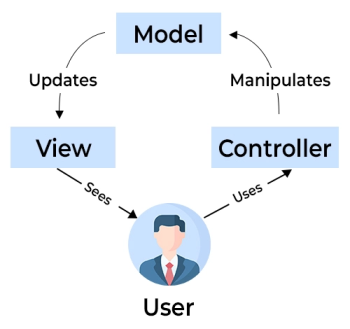
\includegraphics[width=0.5\textwidth]{slike/mvc.png}
            \caption{MVC model}
            \label{fig:mesh1}
        \end{figure}
        
        \textbf{Web preglednik} je program (software) koji omogućava korisnicima pregledavanje i prikazivanje web stranica na World Wide Webu (WWW). Predstavlja sučelje između korisnika i internetskog sadržaja. Pomoću njega korisnik sustava komunicira s web aplikacijom, točnije \textit{View} i \textit{Controller} komponentom.
        
        \pagebreak

        \textbf{Web aplikaciju} pokreće \textbf{poslužitelj}. To je program čiji je osnovni zadatak odgovarati na HTTP (\textit{Hyper Text Transfer Protocol}) zahtjeve klijenata, primati i slati određene resurse - posluživati samu aplikaciju. 
        
        \begingroup 
        U većini slučajeva klijent će zahtjevati pristup podacima kojima web poslužitelj nema pristup. U tom slučaju će \textit{Controller} komponenta poslati zahtjev \textit{Model} komponenti, zaslužnoj za pohranu korisničkih podataka, koju u našem slučaju predstavlja \textbf{baza podataka}. 
        \endgroup
        
        \begingroup
        Baza podataka organizirana je zbirka logički povezanih, pretražljivih i međusobno ovisnih podataka. Ključna je komponenta mnogih aplikacija i sustava zbog mogućnosti sigurne pohrane i brzog pretraživanja SQL upitima.
	  \endgroup

        \begingroup
        Za našu implementaciju korisničkog sučelja odabrali smo programski jezik \textit{JavaScript} s bibliotekom \textit{React}. Za implementaciju poslužiteljske strane odabrali smo programski jezik \textit{Java} i \textit{Spring} framework, točnije proširenje \textit{Spring Boot}. Kao razvojnu okolinu odabrali smo \textit{Visual Studio Code} i \textit{JetBrains IntelliJ IDEA}. Za implementaciju baze podataka odabrali smo \textit{PostgreSQL}.
        \endgroup

		\begin{figure}[h]
            \centering
            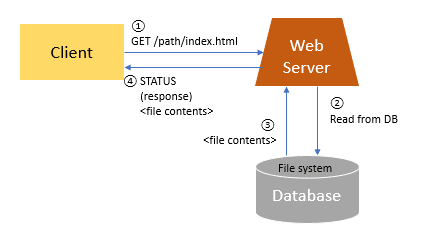
\includegraphics[width=1\textwidth]{slike/client-server-db.png}
            \caption{Prikaz osnovnog rada sustava}
            \label{fig:mesh1}
        \end{figure}

        \pagebreak
				
		\section{Baza podataka}
			
			\textbf{\textit{dio 1. revizije}}\\
			
		\textit{Potrebno je opisati koju vrstu i implementaciju baze podataka ste odabrali, glavne komponente od kojih se sastoji i slično.}
		
			\subsection{Opis tablica}
			

				\textit{Svaku tablicu je potrebno opisati po zadanom predlošku. Lijevo se nalazi točno ime varijable u bazi podataka, u sredini se nalazi tip podataka, a desno se nalazi opis varijable. Svjetlozelenom bojom označite primarni ključ. Svjetlo plavom označite strani ključ}
				
				
				\begin{longtblr}[
					label=none,
					entry=none
					]{
						width = \textwidth,
						colspec={|X[6,l]|X[6, l]|X[20, l]|}, 
						rowhead = 1,
					} %definicija širine tablice, širine stupaca, poravnanje i broja redaka naslova tablice
					\hline \SetCell[c=3]{c}{\textbf{korisnik - ime tablice}}	 \\ \hline[3pt]
					\SetCell{LightGreen}IDKorisnik & INT	&  	Lorem ipsum dolor sit amet, consectetur adipiscing elit, sed do eiusmod  	\\ \hline
					korisnickoIme	& VARCHAR &   	\\ \hline 
					email & VARCHAR &   \\ \hline 
					ime & VARCHAR	&  		\\ \hline 
					\SetCell{LightBlue} primjer	& VARCHAR &   	\\ \hline 
				\end{longtblr}
				
				
			
			\subsection{Dijagram baze podataka}
				\textit{ U ovom potpoglavlju potrebno je umetnuti dijagram baze podataka. Primarni i strani ključevi moraju biti označeni, a tablice povezane. Bazu podataka je potrebno normalizirati. Podsjetite se kolegija "Baze podataka".}
			
			\eject
			
			
		\section{Dijagram razreda}
		
			\textit{Potrebno je priložiti dijagram razreda s pripadajućim opisom. Zbog preglednosti je moguće dijagram razlomiti na više njih, ali moraju biti grupirani prema sličnim razinama apstrakcije i srodnim funkcionalnostima.}\\
			
			\textbf{\textit{dio 1. revizije}}\\
			
			\textit{Prilikom prve predaje projekta, potrebno je priložiti potpuno razrađen dijagram razreda vezan uz \textbf{generičku funkcionalnost} sustava. Ostale funkcionalnosti trebaju biti idejno razrađene u dijagramu sa sljedećim komponentama: nazivi razreda, nazivi metoda i vrste pristupa metodama (npr. javni, zaštićeni), nazivi atributa razreda, veze i odnosi između razreda.}\\
			
			\textbf{\textit{dio 2. revizije}}\\			
			
			\textit{Prilikom druge predaje projekta dijagram razreda i opisi moraju odgovarati stvarnom stanju implementacije}
			
			
			
			\eject
		
		\section{Dijagram stanja}
			
			
			\textbf{\textit{dio 2. revizije}}\\
			
			\textit{Potrebno je priložiti dijagram stanja i opisati ga. Dovoljan je jedan dijagram stanja koji prikazuje \textbf{značajan dio funkcionalnosti} sustava. Na primjer, stanja korisničkog sučelja i tijek korištenja neke ključne funkcionalnosti jesu značajan dio sustava, a registracija i prijava nisu. }
			
			
			\eject 
		
		\section{Dijagram aktivnosti}
			
			\textbf{\textit{dio 2. revizije}}\\
			
			 \textit{Potrebno je priložiti dijagram aktivnosti s pripadajućim opisom. Dijagram aktivnosti treba prikazivati značajan dio sustava.}
			
			\eject
		\section{Dijagram komponenti}
		
			\textbf{\textit{dio 2. revizije}}\\
		
			 \textit{Potrebno je priložiti dijagram komponenti s pripadajućim opisom. Dijagram komponenti treba prikazivati strukturu cijele aplikacije.}